\documentclass[a4paper,11pt,oneside,titlepage,openany,onecolumn]{scrreprt}

%%%%%%%%%%%%%%%%%%%%%%%%%%%%%%%%%%%%%%%%%%%%%%%%%%%%%%%%%%%%%%%%%%%%%%%%%%%%%%%%%%%%%%

\usepackage{ifthen}
\newboolean{english}
\setboolean{english}{true}


\def\title{Development of a vibrotactile stimulation system for cognitive rehabilitation}
\def\study{Mechatronics \& Smart Technologies}
\def\thesis{Master Thesis}
\def\degree{"Master of Science in Engineering"}
\def\student{Lukas Sieß}
\def\matnr{52010293}
\def\address{6591 Grins, Grins 107H}
\def\reviewerone{Prof. Yeongmi Kim, PhD}


% deutsche Anpassungen
%\usepackage[ansinew]{inputenc}
\usepackage[T1]{fontenc}
\usepackage[ngerman,english]{babel}
%\usepackage{babelbib}

% mathematische Symbole
\usepackage{amsmath,amssymb,amsfonts,amstext}

% Listings
\usepackage{listings}
\lstset{numbers=left,numberstyle=\tiny,stepnumber=5,numbersep=5pt}

% erweiterte Zeichenbefehle
\usepackage{pst-all}

% Kopfzeilen frei gestaltbar
\usepackage{fancyhdr}
\lfoot[\fancyplain{}{}]{\fancyplain{}{}}
\rfoot[\fancyplain{}{}]{\fancyplain{}{}}
\cfoot[\fancyplain{}{\footnotesize\thepage}]{\fancyplain{}{\footnotesize\thepage}}
\lhead[\fancyplain{}{\footnotesize\nouppercase\leftmark}]{\fancyplain{}{}}
\chead{}
\rhead[\fancyplain{}{}]{\fancyplain{}{\footnotesize\nouppercase\sc\leftmark}} 

% Farben im Dokument m"oglich
\usepackage{color}

% Schriftart Helvetica
\usepackage{helvet}
\renewcommand{\familydefault}{phv}

% anderdhalbfacher Zeilenabstand
\usepackage{setspace}
\onehalfspacing

% Graphiken einbinden: hier f"ur pdflatex
\usepackage[dvips]{graphicx}

% verbesserte Floating Plazierung
\usepackage{float}

% "Uberpr"ufung des Layouts
\usepackage{layout}

\usepackage{array}

% erweiterte Einstellungen der Bildunterschriften -> 8 Pt
\usepackage[small]{caption}
\captionsetup{belowskip=12pt,aboveskip=4pt}

\usepackage{ifthen}

% H"ohe und Breite des Textk"orpers etwas gr"osser definieren
\usepackage[tmargin=1in,bmargin=1in,lmargin=1.25in,rmargin=1.25in]{geometry}

% Einr"uckung von und Abstand zwischen Abs"atzen
\setlength{\parindent}{0em}
\setlength{\parskip}{1.5ex plus0.5ex minus0.5ex}

% weniger Warnungen wegen "uberf"ullter Boxen
\tolerance = 9999
\sloppy

% Anpassung einiger "Uberschriften 
\renewcommand\figurename{Abbildung}
\renewcommand\tablename{Tabelle}
%\newcommand{\unit}{\mathrm}

% Counter f"ur die Nummerierung
\newcounter{romancount}

% Boolsche Variable f"ur Bachelor-/Masterarbeit oder Bericht
\newboolean{thesis}


\begin{document}

\ifthenelse{\boolean{english}}{\selectlanguage{english}}{\selectlanguage{english}}

%\layout

% Kopf- und Fusszeilen initiieren
\pagestyle{plain}

\pagenumbering{Roman}
\thispagestyle{empty}
\sffamily

\ThisTileWallPaper{\paperwidth}{\paperheight}{Images/MCIHintergrundKPL.pdf}
%\put(-30,-685){\includegraphics[width=1.15\linewidth]{BG}}

{
	\bfseries

	\vspace*{3.5cm}

	\textcolor{MSBlue}{\sffamily\bfseries\huge\thesis}%

	\vspace*{0.5cm}

	\begin{doublespace} 
		
\textbf{\labtitle{} (\labcode)}

\textbf{\labname}

\textbf{\labdate}	

%Labor \labnum

	%\maketitle
	\vspace*{10cm}

	\textcolor{gray}{\study}

	\def\termname{Semester}
	\textcolor{gray}{\term{ }\termname}

	\def\lecturername{Lector}
	\textcolor{gray}{\lecturername: \lecturer}

	\def\groupname{Group}
	\textcolor{gray}{\groupname: \group}

	\def\authorname{Authors}
	\textcolor{gray}{\authorname: \student}

	\textcolor{gray}{\today}
	\end{doublespace} 
	\newpage
}
\ifthenelse{\boolean{english}}
{\section*{\centering Declaration in Lieu of Oath}
\glqq I hereby declare, under oath, that this \MakeLowercase{\thesis} has been my independent work and has not been aided with any prohibited means. I declare, to the best of my knowledge and belief, that all passages taken from published and unpublished sources or docments have been reproduced whether as original, slightlychanged or in thought, have been mentioned as such at the corresponding placesof the thesis, by citation, where the extend of the original quotes is indicated.\grqq\\[5\baselineskip]
\rule{5cm}{0.2pt}\hfill\rule{5cm}{0.2pt}\\
\phantom{Date }Place, Date\hfill Signature\hspace{15mm}}
{\section*{\centering Eidesstattliche Erkl"arung}
\glqq Ich erkl"are hiermit an Eides statt, dass ich die vorliegende Arbeit selbst"andig angefertigt habe. Die aus fremden Quellen direkt oder indirekt "ubernommenen Gedanken sind als solche kenntlich gemacht. Die Arbeit wurde bisher weder in gleicher noch in "ahnlicher Form einer anderen Pr"ufungsbeh"orde vorgelegt und auch noch nicht ver"offentlicht.\grqq\\[5\baselineskip]
\rule{5cm}{0.2pt}\hfill\rule{5cm}{0.2pt}\\
\phantom{Datum }Ort, Datum\hfill Unterschrift\hspace{15mm}}
\newpage

\section*{\centering \ifthenelse{\boolean{english}}{Acknowledgement}{Danksagung}}
Text Text Text Text Text Text Text Text Text Text Text Text Text Text Text Text Text Text Text Text Text Text Text Text ...
\newpage

\selectlanguage{ngerman}
\section*{\centering Kurzfassung}
Text Text Text Text Text Text Text Text Text Text Text Text Text Text Text Text Text Text Text Text Text Text Text Text ...

% Bitte 3-5 deutsche Schlagw"orter eingeben, die die Arbeit charakterisieren:
\paragraph*{Schlagw"orter:} Schlagwort 1, Schlagwort 2, Schlagwort 3, Schlagwort 4, Schlagwort 5
\newpage

\selectlanguage{english}
\section*{\centering Abstract}
Text Text Text Text Text Text Text Text Text Text Text Text Text Text Text Text Text Text Text Text Text Text Text Text ...

% Bitte 3-5 englische Keywords eingeben, die die Arbeit charakterisieren:
\paragraph*{Keywords:} Keyword 1, Keyword 2, Keyword 3, Keyword 4, Keyword 5

\newpage


\ifthenelse{\boolean{english}}{\selectlanguage{english}}{\selectlanguage{english}}

\tableofcontents%\thispagestyle{empty}
\newpage

\setcounter{romancount}{\value{page}}
\setcounter{page}{1}
\pagenumbering{arabic}

% Kopf- und Fusszeilen initiieren
\pagestyle{fancy}

\selectlanguage{english}

\chapter[Introduction]{Introduction}

\section{Motivation and Problem Statement}

F"uhren Sie an dieser Stelle zur Arbeit hin und erkl"aren Sie die Hintergr"unde welche der Themenstellung ihre besondere Relevanz verleiht.

\section{Objectives of the Thesis}

Erl"autern Sie an dieser Stelle \emph{genau} was ihre Aufgabe ist. Gegebenfalls grenzen Sie auch die Teile aus, welche nicht im Umfang der Arbeit liegen. Dies kann Ihnen gegen Ende ihrer Arbeit bei der Argumentation helfen.

\section{Structure of the Thesis}

Geben Sie in diesem Abschnitt eine grobe Vorausschau auf den Aufbau der Arbeit. Die Arbeit k"onnte empirisch motiviert sein und mit der Auswertung eines Experimentes beginnen oder theoreitsch und somit logischerweise mit einem Theoriekapitel beginnen.

\chapter[Theoretical Background]{Theoretical Background}

\section{Cognitive Rehabilitation: Concepts, Methods, and Target Groups}
Multidisziplinäre Ansätze
\cite{Zucchella.2018}
EEG-Biomarker wie der Brain Symmetry Index (BSI) und der Laterality Coefficient (LC) erlauben eine objektive Bewertung des funktionellen Zustands des Gehirns. Die EEG-Analyse ermöglicht eine individualisierte Rehabilitationssteuerung, indem sie Veränderungen in der Hirnaktivität erfasst – insbesondere im Zusammenhang mit Motor Imagery, einer etablierten kognitiven Rehabilitationsmethode.
Die Zielgruppe der Studie sind Schlaganfallpatienten, die oft sowohl motorische als auch kognitive Beeinträchtigungen aufweisen.



% Campbell Review
\cite{Campbell.2022}
    
\begin{table}[htp]
	\centering
	\caption[Vergleich verschiedener Studien zur taktilen niederfrequenten Vibration in der Demenzbehandlung1]{ergleich verschiedener Studien zur taktilen niederfrequenten Vibration in der Demenzbehandlung}
	\label{tab:TLFV_Demenz}
	\footnotesize
    \resizebox{0.1\linewidth}{!}{
	%\resizebox{.5\textwidth}{!}{
		\begin{tabular}{r c c c l}
			\toprule
			Studie (Autor, Jahr) & Vibrationsart & Dauer / Häufigkeit & Ergebnisse & Anwendungskontext\\
            \midrule
            Clements-Cortes et al., 2016 & Vibroakustisch (40 Hz, Musik, physioakustischer Stuhl) & 2x/Woche, 6 Wochen & Verbesserte SLUMS-Werte, mehr Aufmerksamkeit & Ambulante Einrichtung \\
            Clements-Cortes et al., 2017a & Vibroakustisch (40 Hz, tägliche Heimanwendung) & Täglich, 3 Jahre & Stabile MMSE-Werte über 3 Jahre, reduzierte Frustration & Heimanwendung \\
            Kim und Lee, 2018 & Mechanisch (WBV, Frequenzsteigerung von 20–35 Hz) & 5x/Woche, 8 Wochen & Signifikante EEG-Aktivierung, kognitive Verbesserung & Gemeindezentren \\
            Lam et al., 2018 & Mechanisch (WBV, 30 Hz, 2 mm Amplitude) & 2x/Woche, 9 Wochen & Verbesserte Mobilität, Gleichgewicht, hohe Teilnahmequote & Tagespflege \\
            Heesterbeek et al., 2019a & Mechanisch (WBV, 30 Hz, 1–2 mm Amplitude) & Mehrfach/Woche, Dauer 12 Min & Gute Akzeptanz, einige berichtete Übelkeit & Pflegeheim \\
			\bottomrule
		\end{tabular}
		}
\end{table}

\section{Vibrotactile Stimulation: Principles and Therapeutic Applications}
%Vibrotactile Stimulation
\cite{Campbell.2022}

\cite{ClementsCortes.2016, Heesterbeek.2019,Lam.2018, Clair.1993, Kim.2018, ClementsCortes.2017, Mercado.2006, ClementsCortes.2017b, ClementsCortes.2022}


\section{Actuation Technologies for Haptic Feedbacks}

\section{Voice Coil Actuators for Vibrotactile Stimulation}

\section{Overview of Existing Vibrotactile Stimulation Systems}


[14]–[22] zeigen Wirksamkeit bei AD
%2.3 40 Hz & Gamma Frequenzen	[9], [10], [11], [12] zeigen neurobiologische Wirkung
%2.4 EEG & Wearables	[4]–[8] über EEG-Tech, BCI, und mobile Erfassung
%2.5 VCAs (selbst ergänzt)	Hier kannst du technische Quellen ergänzen, z. B. Datenblätter oder Paper zu haptischen Aktuatoren
\chapter{Analysis of the Current VCA-Based System}

\section{Hardware Components (Voice Coil Actuators, Control Electronics, Sensors)}

\section{Software Architecture and Control Strategies}

\section{Limitations and Identified Challenges}

\chapter[Formatierungen]{Formeln}\label{cha-formeln}

Ein besonderer Vorteil von \LaTeX ist die schnelle und einfache Art Formeln einzugeben. Mit ein wenig "Ubung in der Nomenklatur gehen die komplexesten Ausdr"ucke problemlos von der Hand. Eine einfache Formel sieht folgendermaßen.
\begin{equation}
p_1+\frac{\rho v_1^2}{2}+\rho gh_1=p_2+\frac{\rho v_2^2}{2}+\rho gh_2+\Delta p.
\label{eqn-bernoulli}
\end{equation}
Oft ziehen sich Formeln "uber mehrere Zeilen  
\begin{eqnarray}
\Delta L&=&\int\limits_0^L(1-\cos\varphi)\,dx\approx\int\limits_0^L[1-(1-\varphi^2/2)]\,dx=\frac{1}{2}\int\limits_0^Lw'^2\,dx=\nonumber\\
&=&\frac{B^2\lambda^2}{2}\int\limits_0^L\cos^2\lambda x\,dx=\frac{B^2\lambda^2}{2}\left[\frac{\lambda x-\sin\lambda x\cos\lambda x}{2\lambda}\right]_0^L\approx\frac{B^2\lambda^2L}{4}
\end{eqnarray}
oder sind sehr kompliziert
\begin{eqnarray}
\boldsymbol{\tau}&=&2\mu\mathbf{D}=\mu[\nabla\vec{v}+(\nabla\vec{v})^T]\\
\boldsymbol{\sigma}'&=&\mu'\nabla\cdot\,\vec{v}\,\mathbf{I}=-\frac{2}{3}\mu\,\nabla\cdot(\nabla{v})\,\mathbf{I}.
\end{eqnarray}


\chapter{Referenzen und Zitate}\label{cha-ref}

Im Prinzip kann in \LaTeX auf alles referenziert werden was ein Label hat. Dies kann ein Kapitel oder Abschnitt sein, siehe Kapitel \cref{cha-ref} und Anhang \cref{app-A}, eine Formel wie die von Bernoulli \cref{eqn-bernoulli}, eine Graphik wie Abbildung \cref{fig:test_plot_1}, eine Tabelle wie  oder sogar Punkte einer Aufzählung, vgl.~\cref{enum-ebene}.

Noch eleganter sind Zitate. Man zitiert am besten auf ein Kürzel welches sich aus den ersten Buchstaben des Erstautors und der Jahreszahl zusammensetzt wie \cite{Sensoren}. Die Seitenzahl kann als Option angegeben werden \cite{Sensoren}. Verwenden Sie BibTeX, so erscheinen nur die verwendeten Literaturstellen im Literaturverzeichnis und überdies kümmert sich dann \LaTeX um die richtige Reihenfolge und Formatierung der Quellen - egal ob Buch \cite{Sensoren}, Artikel oder Dokumentation \cite{Sensoren}.

\begin{figure}[!ht]
	\centering
	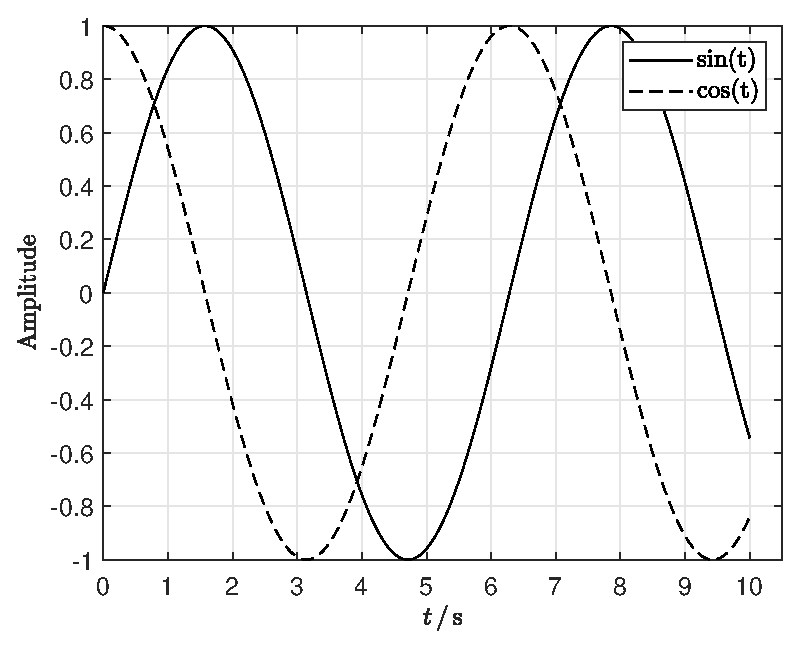
\includegraphics[width=0.6\textwidth]{img/Test_plot_1.eps}
	\caption[60\,\% der Textbreite]{Sinus- und Cosinus-Verlauf über die Zeit dargestellt.}
	\label{fig:test_plot_1}
\end{figure}

Hier ein Beispiel für Zahlen:
\begin{itemize}
	\item \num{1234,56}  % Zahl mit Dezimaltrennzeichen
	\item \SI{2}{\meter^{-1}} % Einheit m^-1 ohne Bruch
	\item \SI{1.23e4}{\newton\meter} % Exponenten mit Punkt als Produkt
	\item \SI{1000}{\kilo\ohm} % Tausender ohne Trennzeichen
\end{itemize}


Testen ob die Symbole und die Akronyms richtig funktionieren \gls{sym:C}, oder auch \gls{sym:L}.

A \gls{acr:pcb} is a fundamental component in the electronics industry and is commonly used to mechanically support and electrically connect various electronic components, including \glspl{acr:ic}. The complex impedance of an inductor is given by the formula
\begin{equation}
	Z_\mathrm{L}=\mathrm{i}\omega\gls{sym:L}
	\label{eqn:testgleichung}
\end{equation}
where $\gls{sym:L}$ is the inductance of the inductor.\par 
In \cref{fig:test_plot_1} ist ein Testplot dargestellt. und die Gleichung wird auch referenziert \cref{eqn:testgleichung}
\chapter{Zusammenfassung und Ausblick}

\section{Zusammenfassung}

Fassen Sie die Arbeit zusammen indem Sie auf die wichtigsten Ergebnisse eingehen. Da Sie die Arbeit als bekannt voraussetzen k"onnen, m"ussen Sie nicht auf Details der Vorgehensweise eingehen.

\section{Reflexion und Ausblick}

Hier k"onnen Sie "uber die Erreichung der Ziele, ihren pers"onlichen Lerneffekt und die Wichtigkeit des Erreichten reflektieren. Die Formulierung eines Ausblicks auf weitere notwendige Arbeiten zeigt, dass Sie sich stark mit dem Inhalt identifizieren.


\selectlanguage{english}

% Literaturverzeichnis IEEE-gerecht
\bibliographystyle{IEEEtran}	
\bibliography{Literatur}
\ifthenelse{\boolean{english}}{\addcontentsline{toc}{chapter}{Bibliography}}{\addcontentsline{toc}{chapter}{Literaturverzeichnis}} % f"ugt den Eintrag "Abbildungsverzeichnis" im Inhaltsverzeichnis hinzu

\pagenumbering{Roman}
\setcounter{page}{\value{romancount}}

\newpage

% Abbildungsverzeichnis
\listoffigures
\ifthenelse{\boolean{english}}{\addcontentsline{toc}{chapter}{List of Figures}}{\addcontentsline{toc}{chapter}{Abbildungsverzeichnis}} % f"ugt den Eintrag "Abbildungsverzeichnis" im Inhaltsverzeichnis hinzu
\newpage

% Tabellenverzeichnis
\listoftables 
\ifthenelse{\boolean{english}}{\addcontentsline{toc}{chapter}{List of Tables}}{\addcontentsline{toc}{chapter}{Tabellenverzeichnis}} % f"ugt den Eintrag "Tabellenverzeichnis" im Inhaltsverzeichnis hinzu
\newpage

% Symbolverzeichnis
\ifthenelse{\boolean{english}}{\addchap{List of Symbols}}{\addchap{Symbolverzeichnis}}
\begin{center}
\hspace{-17mm}\begin{tabular}{>{\raggedleft}p{0.08\linewidth} p{0.3\linewidth} >{\raggedleft\arraybackslash}p{0.2\linewidth}}
\ifthenelse{\boolean{english}}{symbol}{Symbol} &
\ifthenelse{\boolean{english}}{name}{Bezeichnung} & \ifthenelse{\boolean{english}}{unit}{Einheit} \\\hline
$a$ & \ifthenelse{\boolean{english}}{acceleration}{Beschleunigung} & $\unit{\frac{m}{s^2}}$\\
$F$ & \ifthenelse{\boolean{english}}{force}{Kraft} & $\unit{N}$
\end{tabular}
\end{center}

% Abk"urzungsverzeichnis
\ifthenelse{\boolean{english}}{\addchap{Abbreviations}}{\addchap{Abk"urzungsverzeichnis}}
\hspace{-17mm}\begin{tabular}{>{\raggedleft}p{0.2\linewidth} p{0.75\linewidth} p{0.1\linewidth}}
www & World Wide Web \\
URL & Uniform Resource Locator
\end{tabular}


% Anh"ange
\selectlanguage{english}
\begin{appendix}
	\chapter[Erster Anhang]{"Uberschrift des ersten Anhangs}\label{app-A}

Text Text Text Text Text Text Text Text Text Text Text Text Text Text Text Text Text Text Text Text Text Text Text Text ...


	\chapter[Erster Anhang]{"Uberschrift des ersten Anhangs}\label{app-A}

Text Text Text Text Text Text Text Text Text Text Text Text Text Text Text Text Text Text Text Text Text Text Text Text ...


\end{appendix}

\end{document}
